%-----------------------------------------------
% DOCUMENT PACKAGES
%-----------------------------------------------
\documentclass[10pt]{article}
\usepackage[utf8]{inputenc}
\usepackage[T1]{fontenc}
\usepackage{graphicx}
\usepackage[margin=1.3in]{geometry}
\usepackage{hyperref}
\usepackage[french]{babel}
\usepackage[small, sc, bf, center]{titlesec}
\usepackage{listings}
\usepackage{amsmath, amssymb, mathtools}
\usepackage{cleveref}
\usepackage[table]{xcolor}
\usepackage{fancyhdr}
\usepackage{tikz}
\usepackage{tkz-graph}
\usepackage{csvsimple}
%\usepackage{subcaption}
%\usepackage{multicol}
%-----------------------------------------------
% DOCUMENT CONFIG
%-----------------------------------------------

% Add point after title number
\titleformat{\section}[block]{\sc\bfseries\center\large}{\thesection.}{0.5em}{}
\titleformat{\subsection}[block]{\sc\bfseries\center}{\thesubsection.}{0.5em}{}
\titleformat{\subsubsection}[block]{\sc\bfseries\center}{\thesubsubsection.}{0.5em}{}
% Page number reformat
\pagestyle{fancy}
\fancyfoot[C]{--~\thepage~--}
% Deactivate fancyhdr header
\renewcommand{\headrulewidth}{0pt}
\fancyhead{}
% tikz
\tikzstyle{vertex}=[circle, draw, inner sep=0pt, minimum size=6pt]
\newcommand{\vertex}{\node[vertex]}
\usetikzlibrary{arrows,petri,topaths,calc}
% listing style
\lstset{
frame=single,
basicstyle=\ttfamily\small,
numbers=left,
%numbersep=5pt,
%font=\ttfamily
}

%-----------------------------------------------
% DOCUMENT BODY
%-----------------------------------------------
\begin{document}
	
\begin{center}
	\textbf{Projet de résolution de problèmes\\[.5cm]Metaheuristiques pour la résolution du\\problème de l'arbre de
	Steiner de poids minimum}\\[.5cm]
	\textit{Alexandre Bontems, Gualtiero Mottola}\\
	
\end{center}

\tableofcontents

\section{Introduction}
	Ce projet aborde la résolution du problème de l'arbre de Steiner de poids minimum avec deux méthodes: un algorithme génétique et un algorithme de recherche locale. Le problème d'optimisation combinatoire consiste en la recherche d'un arbre de poids minimum couvrant les nœuds dits terminaux d'un graphe. La solution peut comprendre des nœuds facultatifs, dits de Steiner, pour être fortement connexe. La~\Cref{fig-ex1} montre une solution optimale en bleu qui comprend les noeuds de Steiner $u_1$ et $u_2$. 
	
	\begin{figure}[h!]
		\centering
		\begin{tikzpicture}[scale=0.75, transform shape]
			\tikzstyle{edgesol}=[draw=blue!50]
			\tikzstyle{termvertex}=[fill=black]
			% Noeuds terminaux
			\vertex[termvertex] (v1) at (-1,3) [label=above:$v_1$] {};
			\vertex[termvertex] (v2) at (4,3) [label=above:$v_2$] {};									\vertex[termvertex] (v3) at (-0.5,0) [label=below:$v_3$] {};
			\vertex[termvertex] (v4) at (4,-1) [label=below:$v_4$] {};
			\vertex[termvertex] (v5) at (6,-.5) [label=right:$v_5$] {};
			% Noeuds de steiner
			\vertex (u1) at (1.5,2) [label=left:$u_1$] {};
			\vertex (u2) at (3,1) [label=right:$u_2$] {};
			\vertex (u3) at (-2.5,1.5) [label=left:$u_3$] {};
			\vertex (u4) at (6.5,1.5) [label=right:$u_4$] {};
			
			\path
			% Solution
			(v1) edge[edgesol] node[fill=white]{$2$} (u1)
			(u1) edge[edgesol] node[fill=white]{$1$} (u2)
			(v3) edge[edgesol] node[fill=white]{$4$} (u2)
			(u1) edge[edgesol] node[fill=white]{$2$} (v2)
			(v2) edge[edgesol] node[fill=white]{$5$} (v5)
			% Reste des arcs
			(v1) edge node[fill=white]{$2$} (u3)
			(u3) edge node[fill=white]{$8$} (v3)
			(v1) edge node[fill=white]{$9$} (v3)
			(v3) edge node[fill=white]{$8$} (v4)
			(u2) edge node[fill=white]{$3$} (v4)
			(v1) edge node[fill=white]{$8$} (v2)
			(v2) edge node[fill=white]{$8$} (u4)
			(u4) edge node[fill=white]{$8$} (v5)
			(u2) edge node[fill=white]{$5$} (v5)
			;
		\end{tikzpicture}
		\caption{Exemple de Steiner Tree Problem}
		\label{fig-ex1}
	\end{figure}
	
	L'algorithme génétique a été conçu de façon modulaire et peut accueillir différentes fonctions d'initialisation, opérateurs de croisement et de mutation, etc. Il a ainsi été possible d'étudier les performances de chaque composante pour les différentes types d'instances considérés. L'algorithme de recherche locale réutilise les mêmes fonctions d'initialisation.
	
\section{Algorithme génétique}
	Un algorithme génétique consiste généralement en l'enchaînement des actions suivantes sur plusieurs générations: \textit{Initialisation, Sélection, Crossover, Mutation}. La phase d'initialisation permet de générer une population d'individus qui seront ensuite sélectionnés, croisés, et mutés afin de construire la génération suivante.

	\subsection{Population initiale}
		Les individus solutions sont représentés par un vecteur de variables binaires pour chaque sommet facultatif, prenant la valeur $1$ si le sommet est présent dans la solution et 0 sinon. Par exemple, la solution de l'exemple en~\Cref{fig-ex1} est représenté par le vecteur suivant.
		\begin{figure}[h!]
			\centering
			\begin{tabular}{|c|c|c|c|}
				\hline
				$u_1$ & $u_2$ & $u_3$ & $u_4$ \\
				\hline
				1 & 1 & 0 & 0 \\
				\hline
			\end{tabular}
		\end{figure}
	
		\paragraph{Initialisation aléatoire}{
			Une première approche pour la phase d'initialisation a été de produire des individus en choisissant, de manière aléatoire, les sommets pris dans la solution. Les proportions de sommets pris dans une solution sont tirées aléatoirement entre 5 et 20\% lors de la génération d'un individu. On essaye ainsi de se rapprocher le plus possible de l'optimum tout en s'assurant une certaine diversité dans la population de départ.
			
			La~\Cref{tab-randominit} montre des coûts de départ pour quelques instances. Il apparaît qu'ils se trouvent souvent bien loin des solutions optimales et c'est pourquoi on utilisera par la suite des heuristiques de construction. Le temps de résolution étant borné à 5 minutes, on essaye ainsi d'améliorer les performances de nos algorithmes. Cette méthode de génération reste cependant intéressante pour introduire de la diversité dans nos population initiales. Elle sera désignée par \texttt{random} dans la suite de ce rapport.
			
			\begin{table}[h!]
				\centering
				\begin{tabular}{|c|c|c|c|c|}
					\hline
					\textbf{Génération} & \textbf{Instance} & \textbf{Proportion} & \textbf{Coût} & \textbf{Opt} \\
					\hline
					1&b02  & 0.31 & 5075 & 83 \\
					2&b02  & 0.45 & 3602 & 83 \\
					3&b02  & 0.35 & 3102 & 83 \\
					1&b08  & 0.40 & 5112 & 104 \\
					2&b08  & 0.47 & 5180 & 104 \\
					3&b08  & 0.36 & 3174 & 104 \\
					1&c18  & 0.46 & 312 & 113 \\
					2&c18  & 0.44 & 302 & 113 \\
					3&c18  & 0.31 & 238 & 133 \\
					\hline
				\end{tabular}
				\caption{Exemple de population initiale aléatoire}
				\label{tab-randominit}
			\end{table}
			}
		\paragraph{Heuristique du plus court chemin}{
			L'heuristique de construction du plus court chemin (\texttt{shortest\_path}) reste la plus efficace en terme de coût initial. Elle consiste en la construction d'un arbre couvrant depuis le graphe des distances des sommets terminaux. Puisqu'elle est déterministe, on procède avant la génération à une randomisation du graphe problème pour obtenir davantage d'individus différents.
		
		La~\Cref{tab-spinit} présente les coups obtenus grâce à cette heuristique pour quelques instances. Le graphe d'origine est altéré de 5 à 20\% pour chaque poids mais il est évident que la perturbation de l'heuristique est faible: les solutions générées sont souvent identiques.
		
		\begin{table}[h!]
				\centering
				\begin{tabular}{|c|c|c|c|}
					\hline
					\textbf{Génération} & \textbf{Instance} & \textbf{Coût} & \textbf{Opt} \\
					\hline
					1 & b02  & 92 & 83 \\
					2 & b02  & 94 & 83 \\
					3 & b02  & 92 & 83 \\
					1 & b08  & 113 & 104 \\
					2 & b08  & 113 & 104 \\
					3 & b08  & 113 & 104 \\
					1 & c18  & 137 & 113 \\
					2 & c18  & 142 & 113 \\
					3 & c18  & 139 & 133 \\
					\hline
				\end{tabular}
				\caption{Génération avec \texttt{shortest\_path}}
				\label{tab-spinit}
			\end{table}
		}
		\paragraph{Heuristique de l'arbre couvrant minimum}{
		Cette heuristique (\texttt{mst}), relativement facile à calculer, nous permet d'améliorer la diversité de la population initiale. Le graphe d'origine (randomisé comme précédemment) est réduit au maximum en enlevant successivement les nœuds facultatifs de degré $1$. Les coûts de départ sont généralement moins bons que \texttt{shortest\_path} mais cette heuristique est plus sensible à la randomisation et donne plus d'individus différents. Quelques générations sont présentées en~\Cref{tab-mstinit}.
		
		\begin{table}[h!]
			\centering
			\begin{tabular}{|c|c|c|c|}
				\hline
				\textbf{Génération} & \textbf{Instance} & \textbf{Coût} & \textbf{Opt} \\
				\hline
				1&b02  & 93  &83 \\
				2&b02  & 97   &83\\
				3&b02  & 96  &83 \\
				1&b08  & 111  &104\\
				2&b08  & 107  &104\\
				3&b08  & 107  &104\\
				1&c18  & 224  &133\\
				2&c18  & 210  &133\\
				3&c18  & 209  &133\\
				\hline
			\end{tabular}
			\caption{Génération avec \texttt{mst}}
			\label{tab-mstinit}
		\end{table}
		}
		
		Notre algorithme génétique utilisera donc une population constituée d'individus issus de ces trois méthodes de génération. L'heuristique \texttt{shortest\_path} est très coûteuse pour des graphes avec beaucoup de nœuds terminaux et/ou d'arêtes, et elle produit peu d'individus différents malgré la randomisation du graphe de départ. C'est pourquoi seul un faible pourcentage y sera dédié. Par exemple, une population initiale pourra comprendre 5\% de \texttt{shortest\_path}, 60\% d'heuristique de \texttt{mst} et 25\% de \texttt{random}.

	\subsection{Processus de sélection}
		L'étape suivante demande la sélection de plusieurs individus parmi la population courante, à partir desquels seront produits des "enfants" pour constituer la génération suivante. L'idée est de choisir les meilleurs éléments tout en introduisant de l'aléa afin  d'espérer une évolution. Plusieurs processus différents ont été implémenté et testés.
		
		\paragraph{Fitness proportionate selection (\texttt{FPS})}{
			À chaque individu correspond une mesure de fitness ($\frac{1}{\text{coût}}$) qui augmente avec la qualité de la solution et qui nous permet, avec FPS, de choisir les individus selon leur coût. Ceux avec le coût le plus bas auront le plus de chance d'être choisi. Ainsi, l'implémentation est simple: une liste cumulative de fitness est construite, une valeur aléatoire est tirée et un simple parcours de liste permet de choisir un individu. Les performances de ce processus ainsi que des suivants sont détaillés en~\Cref{sec-perf}.
		}
		\paragraph{Stochastic Universal Sampling (\texttt{SUS})}{
			Un autre processus, moins biaisé envers les solutions de grandes fitness, est \texttt{SUS}. Une seule position aléatoire est tirée et les individus sont choisis depuis cette position dans la population selon des intervalles réguliers. On s'assure ainsi que les meilleurs solutions ne soient pas choisies invariablement. Le pseudo-code suivant, trouvé sur Wikipedia, a été implémenté.
			\begin{lstlisting}
F := total fitness of Population
N := number of offspring to keep
P := distance between the pointers (F/N)
Start := random number between 0 and P
Pointers := [Start + i*P | i in [0..(N-1)]]

Keep = list()
for P in Pointers
    i := 0
    while fitness sum of Population[0..i] < P
        i++
    add Population[i] to Keep
return Keep
			\end{lstlisting}
		}
		\paragraph{Tournament Selection (\texttt{TS})}{
		Enfin, un processus de tournoi a été testé: un sous-ensemble de la population est choisi et est trié (par défaut 70\% de la population initiale est choisi aléatoirement). La probabilité pour un individu d'être choisi est ensuite décidée selon le peudo-code suivant.
			\begin{lstlisting}
choose the best individual from the tournament with probability p
choose the second best individual with probability p*(1-p)
choose the third best individual with probability p*((1-p)^2)
and so on
			\end{lstlisting}		
		Puisque les individus sont tirés parmi un sous-ensemble aléatoire de la population, on s'assure ici aussi de ne pas toujours choisir les mêmes solutions. Ainsi les opérateurs de croisement utilisés pourront peut-être mener vers une évolution positive de la population.
		}
	\subsection{Opérateurs de croisement et mutation}
		
		Les individus choisis lors de la sélection sont croisés et mutés avec les opérateurs décrit dans cette section. La nouvelle population est choisie parmi les parents et les enfants par élitisme: 10\% est constituée des meilleurs solutions et le reste est tiré aléatoirement parmi les restants (toujours dans une optique de diversité de la population).
		
		\paragraph{Croisement à point (\texttt{SPC})}{
		L'opérateur de croisement à point unique consiste à choisir une position aléatoire dans les solutions parentes et à intervertir les différentes parties des parents autour de ce point pour produire deux enfants (illustré en~\Cref{fig-spc}).
			\begin{figure}[h!]
				\centering
				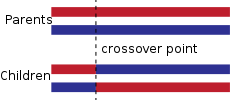
\includegraphics[width=0.3\linewidth]{spc.png}
				\caption{Exemple de croisement à point unique}
				\label{fig-spc}
			\end{figure}
			C'est l'opérateur qui a été le plus prometteur dans nos tests mais beaucoup d'opérateurs souvent utilisés dans les algorithmes génétiques sont absents de ce projet.
		}
		\paragraph{Croisement uniforme (\texttt{UC})}{
		Dans ce croisement, deux enfants sont produits et pour chaque bit d'un enfant, on choisit soit le bit du premier parent soit du second parent à la même position. La probabilité pour chaque bit d'appartenir à un quelconque parent est donc uniforme mais il est très facile d'imaginer une probabilité proportionnelle à la qualité du parent. Malheureusement, par manque de temps, aucune implémentation n'est proposée ici et seul un croisement uniforme a été testé.
		}
		\paragraph{Mutation}{
			Un unique type de mutation a été testé: chaque bit a une probabilité de $\frac{1}{\text{s}}$ d'être modifié avec $s$ le nombre de bits d'une solution. En moyenne on a donc un bit muté par enfant.
		}
	
	\subsection{Performances}
	\label{sec-perf}
	
	Dans ce rapport, tous les algorithmes sont testés sur les ensembles d'instances disponibles à l'adresse \url{http://steinlib.zib.de/testset.php}. Les instances sélectionnées parmi les ensembles $B$, $C$, $D$ et $E$, sont répertoriées en~\Cref{tab-instances}.
	
	\begin{table}[h!]
		\centering
		\begin{tabular}{|c|c|c|c|c|}
			\hline
			\textbf{Nom} & \textbf{Nb de sommets} & \textbf{Nb d'arêtes} & \textbf{Sommets terminaux} & \textbf{Opt} \\
			\hline
			b02 & 50 & 63 & 13 & 83 \\
			b08	& 75 & 94 &	19 & 104 \\
			b10	& 75 & 150 & 13 & 86 \\
			b17	& 100 &	200 & 25 & 131 \\
			b18	& 100 & 200 & 50 & 218 \\
			c02	& 500 & 625 & 10 & 144 \\
			c05	& 500 & 625 & 250 & 1579 \\
			c12	& 500 & 2500 & 10 & 46 \\
			c18 & 500 & 12500 & 83 & 113 \\
			d02	& 1000 & 1250 & 10 & 220 \\
			d04	& 1000 & 1250 & 250 & 1935 \\
			d10	& 1000 & 2000 &	500 & 2110 \\
			e02	& 2500 & 3125 & 10 & 214 \\
			\hline
		\end{tabular}
		\caption{Instances de tests}
		\label{tab-instances}
	\end{table}
	
	    Les performances de l'algorithme génétique sont visibles en~\Cref{tab-perfgen}. Chaque exécution est alloué un maximum de 100 itérations et une population de 100 individus. Les solutions moyennes présentées résultent chacune de 4 exécutions selon les mêmes paramètres. L'opérateur de croisement uniforme donnant des résultats peu satisfaisants, il est absent des mesures de performances dans ce rapport.
	    
	    Pour les instances \textit{b02, b08, b10, b17, b18, c02, c12, d02} et \textit{e02}, les populations initiales sont générées dans les proportions suivantes: 10\% de \texttt{shortest\_path}, 30\% de \texttt{random} et 60\% de \texttt{mst}. Le reste des instances (\textit{c05, c18, d04, d10}) étant trop longues à calculer pour \texttt{shortest\_path}, les populations initiales sont composées de 60\% de \texttt{mst} et 40\% de \texttt{random}.

	\begin{table}[h!]
		\centering
		\begin{tabular}{|c|c|c|c|c|c|c|}
		\hline
\textbf{Instance} & \textbf{Selection} & \textbf{Operator} & \textbf{Avg Time (secs)} & \textbf{Avg Solution} & \textbf{Opt} & \textbf{Error} \\
\hline
\rowcolor{yellow!60} b02 & FPS & SPC & 7.70 & 83 & 83 & 0\% \\
\hline
\rowcolor{yellow!60} b08 & FPS & SPC & 10.38 & 105.5 & 104 & 1.4\% \\
b08 & SUS & SPC & 10.3 & 107 & 104 & 2.8\% \\
b08 & TS  & SPC & 10.4 & 107 & 104 & 2.8\% \\
\hline
\rowcolor{yellow!60} b10 & FPS & SPC & 9.3 & 86 & 86 & 0\% \\
\hline
\rowcolor{yellow!60} b17 & FPS & SPC & 17.4 & 131.5 & 131 & 0.3\% \\
b17 & SUS & SPC & 17.1 & 132 & 131 & 0.7\% \\
\rowcolor{yellow!60} b17 & TS  & SPC & 16.3 & 131.5 & 131 & 0.3\% \\
\hline
c02 & FPS & SPC & 13.3 & 148 & 144 & 2.7\% \\
c02 & SUS & SPC & 13.1 & 148 & 144 & 2.7\% \\
\rowcolor{yellow!60} c02 & TS  & SPC & 26.4 & 147.5 & 144 & 2.4\% \\
\hline
c05 & FPS & SPC & 102.9 & 1598 & 1579 & 1.2\% \\
c05 & SUS & SPC & 102.1 & 1591 & 1579 & 0.7\% \\
\rowcolor{yellow!60} c05 & TS & SPC & 91.5 & 1583.75 & 1579 & 0.3\% \\
\hline
c12 & FPS & SPC & 16.8 & 57.25 & 46 & 24.4\% \\
c12 & SUS & SPC & 19.35 & 58 & 46 & 26\% \\
\rowcolor{yellow!60} c12 & TS & SPC & 23.4 & 56.75 & 46 & 23.3\% \\
\hline
c18 & FPS & SPC & 235.6 & 158.25 & 113 & 40\% \\
c18 & SUS & SPC & 226.8 & 161.25 & 113 & 42.6 \% \\
\rowcolor{yellow!60} c18 & TS & SPC & 160.4 & 119 & 113 & 5.3\% \\
\hline
d02 & FPS & SPC & 25.82 & 233.5 & 220 & 6\% \\
d02 & SUS & SPC & 25.59 & 233.75 & 220 & 6.2\% \\
\rowcolor{yellow!60} d02 & TS & SPC & 50.8 & 232 & 220 & 5.4\% \\
\hline
d04 & FPS & SPC & 157.6 & 2087.75 & 1935 & 7.8\% \\
d04 & SUS & SPC & 149.8 & 2083.75 & 1935 & 7.6\% \\
\rowcolor{yellow!60} d04 & TS & SPC & 132.7 & 2005.75 & 1935 & 3.6\% \\
\hline
d10 & FPS & SPC & 257.3 & 2182 & 2110 & 3.4\% \\
d10 & SUS & SPC & 241.4 & 2185.5 & 2110 & 3.5\% \\
\rowcolor{yellow!60} d10 & TS & SPC & 220.2 & 2130 & 2110 & 0.9\% \\
\hline
e02 & FPS & SPC & 41.2 & 244 & 214 & 14\% \\
e02 & SUS & SPC & 41.4 & 244 & 214 & 14\% \\
e02 & TS & SPC & 108.7 & 244 & 214 & 14\% \\
\hline
		\end{tabular}
		\caption{Performances de l'algorithme génétique}
		\label{tab-perfgen}
	\end{table}
	
	\paragraph{Interprétation}{
	 On se rend compte que le meilleur processus de sélection n'est pas toujours le même et change selon les instances. Si \texttt{FPS} donne les meilleurs résultats pour les instances de type $B$, il est souvent moins bons sur le reste des instances que \texttt{TS} qui règne en maître sur la plupart du tableau. En outre, lors des exécutions des grandes instances (\textit{c12} et \textit{c18} par exemple) beaucoup d'itérations ne montraient pas d'évolution du meilleur coût. Cela est peut être dû à l'opérateur utilisé, plutôt simpliste.
	}
	
	
\section{Recherche locale}

Le patron d'un algorithme de recherche locale est constitué de deux parties. La première étape étant l'initialisation qui nécessite de trouver une solution au problème de manière rapide, grâce à une heuristique par exemple. La seconde étape consiste ensuite à générer une ou plusieurs solutions voisines à partir de la solution précédente et en choisir une parmi celles-ci. On répète ensuite ce procédé jusqu'à une condition d'arrêt.

\subsection{Implémentation}
Pour la génération de la solution initiale, nous avons utilisé les heuristiques de construction décrites précédemment, (\texttt{shortest\_path} et \texttt{mst}). Les solutions voisines sont générées de la façon suivante : les nœuds non terminaux du graphe sont parcourus par ordre d'apparition, si le nœud fait parti de la solution courante (bit à $1$), alors on enlève ce dernier de la solution et on recalcule le score du nouveau graphe. Inversement si le nœud ne fait pas parti de la solution courante (bit a $0$), alors si celui-ci est lié par plus de deux arêtes a un des sommets de la solution courante, on l'ajoute et on recalcule le score.
    Si le score de la nouvelle solution est supérieur à celui de l'ancienne, alors cette nouvelle solution devient la solution courante. Cette étape est répétée jusqu'à ce qu'on ne puisse plus trouver de solution améliorante.

    
\subsection{Performances}

	Les performances de la recherche locale sont visibles en~\Cref{tab-perfls}. Pour chaque instance sélectionnée parmi \textit{b02, b08, b10, b17, c02, c12, d02, et e02}, nous générons les solution initiales avec les trois différentes méthodes de génération : \texttt{shortest\_path}, \texttt{mst} et \texttt{random}. Pour chacune des heuristiques l'algorithme de recherche locale est lancé trois fois, chaque ligne correspond donc a une moyenne sur 3 exécutions. Les données récupérées sont donc les suivantes: le score moyen avant la recherche locale (Init. Score), le nombre d'itération moyen de la recherche de voisins (Avg Iter.), la valeur moyenne de la solution après l'exécution de l'algorithme (Avg Sol.), et enfin le temps d'exécution moyen (Avg Time). 
	\begin{table}[h!]
		\centering
		\begin{tabular}{|c|c|c|c|c|c|c|c|}
		\hline
\textbf{Inst.} & \textbf{Heuristic} & \textbf{Init. \linebreak Score} & \textbf{Avg Iter.} & \textbf{Avg Sol.} & \textbf{Avg Time} & \textbf{Opt} & \textbf{Err.} \\
\hline
b02 & random & 4 416,33 & 15,33 & 255,67 & 0,06 & 83,00 & 208,03\% \\
b02 & shortest & 97,00 & 3,00 & 89,00 & 0,04 & 83,00 & 7,23\% \\
\rowcolor{yellow!60} b02 & mst & 96,00 & 2,33 & 83,00 & 0,02 & 83,00 & 0,00\% \\
\hline
b08 & random & 5 796,33 & 26,67 & 107,33 & 0,21 & 104,00 & 3,21\% \\
\rowcolor{yellow!60} b08 & shortest & 113,00 & 2,00 & 104,00 & 0,03 & 104,00 & 0,00\% \\
b08 & mst & 108,67 & 0,67 & 107,33 & 0,00 & 104,00 & 3,21\% \\
\hline
b10 & random & 4 289,67 & 29,33 & 250,00 & 0,33 & 86,00 & 190,70\% \\
b10 & shortest & 114,00 & 7,67 & 90,33 & 0,07 & 86,00 & 5,04\% \\
\rowcolor{yellow!60} b10 & mst & 107,33 & 8,67 & 88,67 & 0,15 & 86,00 & 3,10\% \\
\hline
b17 & random & 5 916,00 & 38,33 & 137,00 & 0,90 & 131,00 & 4,58\% \\
\rowcolor{yellow!60} b17 & shortest & 149,33 & 6,00 & 135,00 & 0,15 & 131,00 & 3,05\% \\
\rowcolor{yellow!60} b17 & mst & 144,33 & 4,67 & 135,00 & 0,69 & 131,00 & 3,05\% \\
\hline
c02 & random & 35 694,00 & 228,67 & 811,00 & 24,59 & 144,00 & 463,19\% \\
\rowcolor{yellow!60} c02 & shortest & 148,00 & 0,00 & 148,00 & 0,05 & 144,00 & 2,78\% \\
c02 & mst & 238,33 & 18,67 & 174,67 & 0,96 & 144,00 & 21,30\% \\
\hline
c12 & random & 3 276,00 & 240,00 & 73,33 & 128,33 & 46,00 & 59,42\% \\
c12 & shortest & 74,00 & 5,67 & 62,33 & 0,25 & 46,00 & 35,51\% \\
\rowcolor{yellow!60} c12 & mst & 87,67 & 21,67 & 61,67 & 3,26 & 46,00 & 34,06\% \\
\hline
d02 & random & - & - & - & inf & 220,00 & inf \\
\rowcolor{yellow!60} d02 & shortest & 250,00 & 2,00 & 242,00 & 0,18 & 220,00 & 10,00\% \\
d02 & mst & 352,00 & 21,33 & 287,00 & 1,76 & 220,00 & 30,45\% \\
\hline
e02 & random & - & - & - & inf & 214,00 & inf \\
\rowcolor{yellow!60} e02 & shortest & 249,00 & 0,00 & 249,00 & 0,29 & 214,00 & 16,36\% \\
e02 & mst & 604,00 & 56,00 & 425,33 & 13,54 & 214,00 & 98,75\% \\
\hline
		\end{tabular}
		\caption{Performances de l'algorithme de recherche locale (Temps moyen est en secondes)}
		\label{tab-perfls}
	\end{table}
	
	\paragraph{Interprétation} 
Notre algorithme de recherche locale étant déterministe (dû a l'implémentation de la recherche de voisins) le résultat de l'exécution varie grandement en fonction de la méthode de génération choisie. On remarque en effet, sans surprise, que les performances de la recherche locale sont médiocres lorsque la génération choisie est \texttt{random}. D'une manière générale pour les heuristiques (\texttt{shortest\_path} et \texttt{mst}) la recherche locale converge bien plus rapidement que l'algorithme génétique mais la marge d'erreur par rapport a la solution optimale est supérieure. Des comparaisons sont visibles en~\Cref{tab-perfcomp}.
	
	\begin{table}[h!]
		\centering
		\begin{tabular}{|c|c|c|c|}
		\hline
\textbf{Inst.}& \textbf{Opt} & \textbf{Err. local} &  \textbf{Err. genetique} \\
\hline
b02 & 83,00 & 0,00\% & 0\% \\
b08 & 104,00 & 0,00\% & 1.4\% \\
b10 & 86,00 & 3,10 \% & 0\% \\
b17 & 131,00 & 3,05\% & 0.3\%\\
c02 & 144,00 & 2,78 \% & 2.4\%\\
c12 & 46,00 & 34,06\%& 23.3\% \\
d02 & 220,00 & 10,00\% & 5.4\%\\
e02 & 214,00 & 16,36\% & 14\%\\
\hline
		\end{tabular}
		\caption{comparaison des deux algorithmes}
		\label{tab-perfcomp}
	\end{table}

\section{Conclusion}

	Les implémentations proposées dans ce projet présentent des bonnes bases pour la résolution du Steiner Tree Problem. Il est de notre avis, cependant, que plusieurs améliorations sont possibles. En ce qui concerne l'algorithme génétique, il est évident que des opérateurs supplémentaires doivent être testés. L'analyse préalable des instances données à l'algorithme pourrait également se révéler utile pour décider des composantes les plus appropriées à une exécution donnée (métaheuristiques pour décider des processus de sélection et autres opérateurs). L'algorithme de recherche locale, quant à lui, pourrait tirer à son avantage sa rapidité de convergence: relance sur un autre point de départ. Enfin, une combinaison des deux algorithmes est une piste intéressante pour l'amélioration des performances. Procéder à une recherche locale depuis la solution donnée par l'algorithme génétique permettrait d'évoluer positivement après la convergence génétique. On peut aussi imaginer l'évolution d'une population par recherche locale... Malheureusement le temps nous presse et le développement de ces pistes doit être remis à plus tard.
\end{document}